\RequirePackage[l2tabu,orthodox]{nag}

% TODO: decide if one-sided/two-sided
%\documentclass[headsepline,footsepline,footinclude=false,fontsize=11pt,paper=a4,listof=totoc,bibliography=totoc,BCOR=12mm,DIV=12]{scrbook} % two-sided
\documentclass[headsepline,footsepline,footinclude=false,oneside,fontsize=11pt,paper=a4,listof=totoc,bibliography=totoc]{scrbook} % one-sided

\PassOptionsToPackage{table,svgnames,dvipsnames}{xcolor}

\usepackage[utf8]{inputenc}
\usepackage[T1]{fontenc}
\usepackage[sc]{mathpazo}
\usepackage[american]{babel}
\usepackage[autostyle]{csquotes}
\usepackage[%
  backend=bibtex,
  url=false,
  style=numeric,
  maxnames=4,
  minnames=3,
  maxbibnames=99,
  firstinits,
  uniquename=init]{biblatex} % TODO: adapt bibliography style
\usepackage{graphicx}
\usepackage{scrhack} % necessary for listings package
\usepackage{listings}
\usepackage{lstautogobble}
\usepackage{tikz}
\usepackage{pgfplots}
\usepackage{pgfplotstable}
\usepackage{booktabs}
\usepackage[final]{microtype}
\usepackage{caption}
\usepackage[hidelinks]{hyperref} % hidelinks removes colored boxes around references and links
\usepackage[toc,nonumberlist,acronym]{glossaries} % TODO: remove if glossary not needed
\usepackage{subcaption}
\usepackage{algorithm,algpseudocode}
\bibliography{bibliography/literature}

\setkomafont{disposition}{\normalfont\bfseries} % use serif font for headings
\linespread{1.05} % adjust line spread for mathpazo font

% Settings for glossaries TODO: remove the following block if glossary not needed
\renewcommand{\glsnamefont}[1]{\normalfont\bfseries #1} % use serif font for glossary entry titles
\makeglossaries{}

% Settings for pgfplots
\pgfplotsset{compat=1.9} % TODO: adjust to your installed version
\pgfplotsset{
  % For available color names, see http://www.latextemplates.com/svgnames-colors
  cycle list={CornflowerBlue\\Dandelion\\ForestGreen\\BrickRed\\},
}

% Settings for lstlistings
\lstset{%
  basicstyle=\ttfamily,
  columns=fullflexible,
  autogobble,
  keywordstyle=\bfseries\color{MediumBlue},
  stringstyle=\color{DarkGreen}
}

% Basic information for cover & title page
\newcommand*{\getUniversity}{Technische Universität München}
\newcommand*{\getFaculty}{Fakultät für Informatik}
\newcommand*{\getTitle}{Implementation and Evaluation of a Persuasive Mobile Food Recommendation System}
\newcommand*{\getTitleGer}{Implementierung und Evaluierung eines persuasiven mobilen Ernährungs-Empfehlungssystems}
\newcommand*{\getAuthor}{Muhammad Kabir Khan}
\newcommand*{\getDoctype}{Master's Thesis in Informatics}
\newcommand*{\getSupervisor}{Prof. Johann Schlichter, Ph.D.}
\newcommand*{\getAdvisor}{M.Sc. B\"eatrice Lamche}
\newcommand*{\getSubmissionDate}{June 30, 2015}
\newcommand*{\getSubmissionLocation}{Munich}

% TODO: add custom commands etc.

% TODO: remove if glossary not needed
\newglossaryentry{computer}
{
  name=computer,
  description={is a machine that\ldots}
}

\newacronym{tum}{TUM}{Technische Universität München}


\begin{document}

\begin{titlepage}
  % HACK for two-sided documents: ignore binding correction for cover page.
  % Adapted from Markus Kohm's KOMA-Script titlepage=firstiscover handling.
  % See http://mirrors.ctan.org/macros/latex/contrib/koma-script/scrkernel-title.dtx,
  % \maketitle macro.
  \oddsidemargin=\evensidemargin\relax
  \textwidth=\dimexpr\paperwidth-2\evensidemargin-2in\relax
  \hsize=\textwidth\relax

  \centering

  \vspace{40mm}
  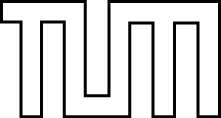
\includegraphics[width=40mm]{logos/tum}

  \vspace{5mm}
  {\huge\MakeUppercase{\getFaculty{}}}\\

  \vspace{5mm}
  {\large\MakeUppercase{\getUniversity{}}}\\

  \vspace{20mm}
  {\Large \getDoctype{}}

  \vspace{15mm}
  {\huge\bfseries \getTitle{}}

  \vspace{15mm}
  {\LARGE \getAuthor{}}

  \vspace{20mm}
  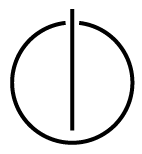
\includegraphics[width=20mm]{logos/faculty}
\end{titlepage}


\frontmatter{}

\begin{titlepage}
  \centering

  \vspace{40mm}
  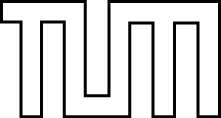
\includegraphics[width=40mm]{logos/tum}

  \vspace{5mm}
  {\huge\MakeUppercase{\getFaculty{}}}\\

  \vspace{5mm}
  {\large\MakeUppercase{\getUniversity{}}}\\

  \vspace{20mm}
  {\Large \getDoctype{}}

  \vspace{15mm}
  {\huge\bfseries \getTitle{}}

  \vspace{10mm}
  {\huge\bfseries \getTitleGer{}}

  \vspace{15mm}
  \begin{tabular}{l l}
    Author: & \getAuthor{} \\
    Supervisor: & \getSupervisor{} \\
    Advisor: & \getAdvisor{} \\
    Submission Date: & \getSubmissionDate{} \\
  \end{tabular}

  \vspace{20mm}
 % 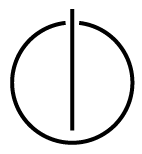
\includegraphics[width=20mm]{logos/faculty}
\end{titlepage}

\thispagestyle{empty}
\vspace*{0.8\textheight}
\noindent
I assure the single handed composition of this \MakeLowercase{\getDoctype{}} only supported by declared resources.

\vspace{15mm}
\noindent
\getSubmissionLocation{}, \getSubmissionDate{} \hspace{5cm} \getAuthor{}

\cleardoublepage{}

\addcontentsline{toc}{chapter}{Acknowledgments}
\thispagestyle{empty}

\vspace*{2cm}

\begin{center}
{\usekomafont{section} Acknowledgments}
\end{center}

\vspace{1cm}

%TODO: Acknowledgments
I would like to thank to my advisor Beatrice Lamche, who always give me her valuable advice and her guide during the phase of my research. I am also very grateful to Geogh Gorh and Silvia Kolssa for there advises in continuing my research.\newline

I also recognize all the participants how took part in user study to evaluate my work. I am also thankful to my dearest friend Muhammad Mudassir Khan for his valuable advices. Least but not the least my family, because of their prayer I would able to make it.

\cleardoublepage{}

\chapter{\abstractname}

%TODO: Abstract



\microtypesetup{protrusion=false}
\tableofcontents{}
\microtypesetup{protrusion=true}

\mainmatter{}

\chapter{Introduction}
\pagenumbering{arabic}%Ab hier, werden arabische Zahlen benutzt
\setcounter{page}{1}%Mit Abschnitt 1 beginnt die Seitennummerierung neu.
\thispagestyle{empty}

The motivation behind this Master Thesis is to implement and evaluate a Healthy Food Recommendation System for Mobile. In the beginning, it provides overview and give the reasoning about the selection of system. Relevant background and related work is presented, Followed by the development and design process together with the evaluation process will be presented. \newline
This chapter will enlighten the motivation behind developed system in Section 1.1. Followed by goals in Section 1.2. Whereas Section 1.3 will provide a brief outline on structure of thesis.

\section{Motivation}\label{motivation}

Rapid innovation and significant advancement in the field of technology and scientific research has made smartphone a primary computing and communication device. Smartphone is now become a necessity of life and people use it as an assistant for their day to day work. According to latest survey more than half of Internet traffic is accounted by mobile device. Enhancement in communication technology and flexible data option provided by network operators has increase relevance of interactive mobile applications. Packed with hundreds of features smartphone use different applications for variety of functionalities which required internet connectivity. Furthermore, smartphone support touch screen and rich support of multimedia and other application take the user experience to the next level.\newline

Suggestions are the important factor of our day-to-day life. From watching a movie, to cooking and to on shopping. We need valuable advice. Recommendations are always helpful in choosing a better alternative. It not only save time but also minimize the individual's effort.\newline

Recommender system are increasingly popular now are days. Form e-comers to movie websites, they not only help to increase business but also behave an personalize user preference assistance. Another aspect of describing Recommend system is filtering technology that user to filter suggests the information to user according to his taste. In order words we can also say that Recommender systems are the smart search engine, which suggest result by, compare different items with each other. Research and advancement are going on this domain in order to improve the quality of recommendations. \newline 
The most important goal for recommendation system designers is user willingness to peruse recommendation provided by the system. Fundamental process of recommendation is finding and conceptualizing relationship of item, current context and how the message is communicated, opens up the way of persuasiveness in recommendations.\newline

Services provided by recommendation system through e-commerce to cooking are numerous in nature. Searching of products returns an overwhelming set of options. For instance, Comparing and Filtering of products among irrelevant set and find the suitable product. Such techniques work fine with web interface, whereas, smartphones they are not very useful due to hardware limitations. Critique-based recommendation helps in revision and acquisition of user preference, in order to improve quality of recommendations.\newline
One the basic need is Food among human. Good health represents proper dietary habit. However, diet plan is always based on person’s physical conditions like gender, weight, age and health status. Furthermore, taste and food preference is differ among individuals. Therefore, creating balance dietary plan based on individuals taste and health preference is always challenging.\newline
The World Health Organization [1] is predicting that the number of obese adults worldwide will reach 2.3 billion by 2015 and the issue is attracting increased attention. Therefore, electronic food management systems have become a hot topic and, are under consideration to replace traditional paper based program. Idea of using electronic devices for health related matter is not new; similar devices are in use by patients for medical reasons e.g. Glucometer, and blood pressure monitor. People want, to carry better life style and to live healthy. Therefore popularity of food monitoring systems is getting popular.  These systems are not only providing valuable services but hold user preferences and keeps history to provide more personalize recommendations. Recommendations are based on food ratings and browsing histories.\newline

Food recommendations have gotten a tremendous amount of success and still in research phase for further improvement. Along with significant advancement and feature set like similar recipes, recipe nutrition detail, where to buy ingredients from some research, some wholes are still remaining. Indeed recommendation techniques like collaborative, content and knowledge based filtering are good for job done. But food domain is not quite simple. User preference and taste not only change by their mood but much more depend upon their health. Therefore, Active learning and critiquing techniques are required to improve better recommendation. So that user can give their feed back and get what ever his preferences are. Mostly approaches are done critiquing by using rating of recipes and generate their result by using celebrative or content based filtering. Similarly, knowledge based filter digs some more; here rating is based on ingredients. Furthermore, persuasion of recommendation is always not guarantied in all cases. Clearly the system is not able to provide the best recommendations due to its detachment from the current situation; what is lacking in these approaches are intersection of persuasiveness, active learning and critiquing and last but not the least user preference context.\newline

This work focuses on generation of health food recommendation on a mobile platform. Recommendation relies on user context, which allow user to critique, based on ingredients and recipes depends on his health and taste through which system will perform active learning. Lastly all recommendations should be persuasive in nature. in order to achieve persuasiveness in recommendations, we focus on user interface and the explanation of recommendation. Which helps user to get an idea why system generates this recommendation to me.\newline

The following short description of the target scenario will illustrate the driving idea behind this research project.\newline

 \textit{John is a software engineer and very health conscious. He has a tight schedule due to work and gym but loves to cook. He wants to keep track of his diet depends on his taste and preferences. Furthermore, he wants try out some new food base on his time schedule}\newline

\section{Goals}

On the basis of scenario, describes in last section, this work reflects the goals which are stated below:\newline
A recommendation is valuable if it interests the user. To determine the generated recommendation is according to user interest entails to our first primary goal, which is offering Persuasive recommendations. Major factors should be considered before given suggestion is Message and Source. Therefore our Second goal is to implement Active Learning and Critiquing approach to justify our suggestion. Since Critiquing relies on context that’s why it is important to understand the Consumption and Accessibility context which infers our third goals.  Similarly understanding the food ontology refers in scenario helps us to understand forth goal of system. Finally how the user will interact with his device conveys our last goals, which is Mobile user interface.\newline

To achieve primary goals there are several other interesting secondary goals, which facilitate, how our primary goals should be achieved. Starting with the research phase, which includes question and answers to user how they want to use such system in order to achieve better usability. Next focus on existing search work how the other system implements food recommendation scenarios, finding out what are their weakness and strengths. Food ontologies understanding how they are interrelate with other. What factor in which recipes are dependent on in order to develop strong system. Understanding user context which time he prefers which recipe. Furthermore, it is important to research on what researches and related work are out there under Persuasive and Active learning and Critiquing system to grab the understanding, how we can get inspiration from their valuable approaches and work. Finally focus on user experience of such application is one of challenging task, how and where to show the important aspects of recipe in our interface, so that it is easy to learn and has improved usability in comparison with current market applications.\newline
Once the research phase has done next step to collect the functional and non-functional requirement of the system, which is collected by interviewing friends and family voluntaries. Once the system is build it has been tested with gathered functional and non-functional requirement and find out the limitation or boundary conditions of system. More over iOS client needs to be test with given requirement additionally user satisfaction should be required for usability test.\newline

Finally, evaluation of developed prototype by user study. In order to clarified the methodologies and processes followed by our selected approaches. After finishing the evaluation reflected results leads to potential improvements and opens up the new direction of research.\newline

\section{Outline}

Division of this thesis is split up into six chapters. \textit{Chapter1} contains introduced the ideas, motivations and goals.\newline

\textit{Chapter2} starts with background in which some definitions and classification of recommendation systems, Followed by different types of profiling and contexts that impact on recommendations. Furthermore, in related work section, pervious work of Persuasiveness, Critiquing and Personalized food recommendation techniques have been discussed.\newline

\textit{Chapter3} explains the Profiling and Context in details along with factors of recommendations. Moreover it covers algorithms that are used to develop the system.\newline

\textit{Chapter4} discuss the System design and architecture phase, which hold the all ERD, components view, servers on which system depend. In the end of the chapter API calls are mentioned which are provided by server.\newline

\textit{Chapter5} elaborates how the user study has been conducted by mentioning the goals, methods, and testing framework along with the dataset. In the end of this chapter measured results and discussion is mention.\newline
  
\textit{Chapter6} will summarizes the achievements and gives clues about further development and research.\newline


\chapter{Background and Related Work}

This chapter will establish the foundation of Persuasive recommendation system along with active learning and critiquing approach. Prior to in depth analysis, it will provide important background information along with some required definitions. Additionally, related work will presented, as the chapter proceed further to the end..\newline

\section{Definitions}

\subsection{Recommender System}

Recommender Systems (RS) are search tools, which supports user decision-making by providing the suggestion that, are according to their interests. Such systems are widely uses from social networking through e-commerce sites in order to achieve different purposed. In e-commerce site, they help not only to serve the customer by suggesting items according to their preferences but also support business to improve in its sale. On the other hand in social network site, to suggest friends or pages like according to user preferences. According to Ricci [Ricci, 2010] "RS are information search tools that have been recently proposed to cope with the "information overload" problem, i.e., the typical state of a web user, of having too much information to make a decision". Proposed solution [Resnick and Varian, 1997] is an intelligent system that suggests the product or service that fulfill the user’s preference in given context or situation. Suggestions provided by such systems are depended on the model how they are keeping information. Majority of RS are typically community based. In this kind of modeling suggestions are depend about item popularity among the user. Where popularity is calculated by ratings. Important question that arise in such systems are to find item accuracy according user preferences. On the other hand Personalized models are used that depends on the various factors which includes user’s preferences, history of bought/liked items, or the items the user has ranked in the past. Various techniques are use in the developing of recommender system. Classification of recommendation systems [Ricci, 2001] will be discussed as follows.

\subsubsection{Content-based filtering}

In this technique recommendations are based on user preference. System recommend items that similar to one is liked by user. Item similarity is calculated by features associated with the compared items [Ricci , 2001]. For example, if a user has rated positively recipe A under the category of sweet then next suggestion that is provided by the system is one which is similar to one user has like before.

\subsubsection{Collaborative-based}

Collaborative filtering is technique in which system find the correlation between item and user based opinions of other users which having a similar taste in past [Shapira , 2001]. Initially system calculates all similar taste users for the current user and calculate the recommended item that contains either rated or liked by other users having similar taste. Importantly in this approach item speciation will not be considered. For instance, if user like recipe A then next recommendation would be recipe that there are other users who liked recipe A also liked recipe B.

\subsubsection{Demographic}

Recommendations are generated according to user demographic profile. Recommendations can be produced for different demographic niches by combining the ratings of users in demographic clusters [Mahmood, 2007]. For example, suggestion provided by the systems are shown according to user’s age. 

\subsubsection{Knowledge-based}

In knowledge-based systems item recommendation is based on domain specific knowledge, which justifies how certain item features meet according to user’s preferences [Ricci , 2001]. Importantly, it uses predication techniques namely Case-based reasoning which reuses the cases past cases that are similar to current case in order to identify item set of recommendation.

\subsubsection{Community-based}

Type of recommendations provided by this kind of system based on preference of user friends. According to Ricci research [Ricci, 2001], People tend to rely more on recommendations provided by friends rather than on recommendations from anonymous individual having similar taste. Such type of RS model relies on user’s social relations including preference of user’s friends. Suggestions depend on rating that is provided by user’s friends.

\subsubsection{Hybrid Recommender Systems}

Hybrid system is a fusion of any two or more techniques motioned above. Ricci [Ricci , 2001] explains the motivation behind such system to avoid the limitation of one technique. For instance, Collaborative filtering have cold startup problem i.e. they are unable to suggest those items, which have no ratings. On the other hand Content-based doesn’t have such limitation by combination of both approach new hybrid system can be formed. Similarly, Burke [Burke, 2007] proposed the combination techniques to create a new hybrid system.

\subsubsection{Traditional Recommender Systems Limitations}

Traditional recommendation approaches focus on the recommending the most relevant item according to user preferences without considering any context information for example place and time. Problem occurs when user interest with the system with a particular context and preference may be change for another context[Adomavicius 
, 2012]. For instance, User wants to cook dinner for his guests expects different recommendations as compared to searching for himself/herself.

\subsection{Contexts}

\subsection{User Profiling}

\subsection{Food Profiling}

\subsection{Conversation Critiquing and Active Learning}

\subsection{Persuasive Recommedations}

\section{Related Work}

\subsection{User's Food Preference Extraction for Personalised Cooking Recipe Recommendation}

\subsection{Knowledge Base Framework for Development of Personalised Food Recommendation System}

\subsection{Interactive Explanations in Mobile Shopping Recommender Systems}

\subsection{Active Learning Strategies for Exploratory Mobile Recommender Systems Interactive Explanations in Mobile Shopping Recommender Systems}
\chapter{Profiling and Contexts}

\section{Profiling}

\subsection{User Profile}
\subsection{Food Profile}

\section{Contexts}

\subsection{Consumption Context}

\subsection{Accessibility Context}

\chapter{System Design and Implementation}

This chapter describes of the system. It starts by providing overview of the system, followed by requirement elicitation to build prototype. Furthermore, it also provide deeper understanding of architectural paradigm by discussing each module and their interconnection.

\section{Overview}

Pervious chapter limits our discussion about the design decision and describe the essential component of the system.  Since the concept is quite abstract and does not dictate any implementation details.  In order to challenge the relevance and capability of the concept, a prototype app, tailored to a real world scenario, should be developed as a “proof of concept”. Our system is divided in to two components: (1) Rest based web application follows modular principle of system design i.e. functionality of a system is divided into multiple concurrent modules. Where coordination of modules depend on database.  Each module has its own Data Access Object (DAO) through with communication take place. Module query existing data with the help of DAO perform their task and update afterward. (2) iOS client provides all the required interface to communicate with the server. It aims to collect information that needs to build user profile and allow active learning and critiquing mechanism to update user profile and increase the trust between user and system by conveying the idea how much system cares about user and his need. 

\section{Requirment elicitation}

This section represents user’s viewpoint of the system. It also describes the purpose of the system by identifying the Functional, non-functional requirements and description of use case in the form of scenarios. It is important to mention here that all the scenarios are developed to evaluate the prototype and are not meant for production purpose. 

\subsection{Functional Requirments}

FoodForMe is a mobile food recommender system that user iOS platform. It purpose to facilitate user to find the food what to cook that matches their personal preferences. Idea behind this prototype application is to proof the concept a combination of Persuasion and critique-based recommender system lead to better recommender and have an impact on user decision making process. Therefore all the functionality in a design is bounded to this purpose. There are two cases of interaction with the system. In case one user need login via Facebook so that system can get its demographic profile instead of asking him to fill out his personal information. Demographic information contains name, birthday, email, name and link of his profile picture. By default system keeps his cooking time preference and course selection preference. User can change these preferences from the setting screen. In second case user can interact without login and having same default preference. As it is notice that some user hesitate to provide their information without having a trust in a system. However, in this particular case user can only view the information. Our rest of discussion will relate do case one.\newline

After getting login and change his preference. User will able to view recipes according to his preference. Each recipe shows the name, star rating, main categories, sub categories, number of reviews and recipe picture. Once the user tap on any recipe, user is able to view detail of selected recipe. Detail screen consists on 3 to 4 sections depends on screen type. Section 1 contains the generic information about the recipe same as discuss above accept it provide large Image of recipe. In Section 2 is related to recipe ingredients, each ingredient item have its name and quantity. Section 3 is about preparation/direction means its guide user how to cook that recipe. Section 4 is an option selection and it will appear as per screen type. In this section system will provide why system think this recipe is according to user preference. User is able to see two screens that display recipes list. First one will display the popular recipes of the system. Recipe course and popularity are the factors on which this will depends on. Motivation behind this to aware user what’s new and hot in system and allow user to change his taste. On the other hand second list will depends only user preference. On detail screen of each recipe system will provide explanation, which tells user what system will think about him and why these recipe recommend to him. \newline

On the detail screen of selected recipe user can criticized on showed item. User can critique on list of indigents by mentioning them he like that ingredient or not. Also he might be able to critique on recipe by given star according to his choice. Additional system allow user to change his personal preferences these include cooking time and course selection. \new 


\subsection{Non Requirments}

From usability to performance aspect of a system Non-functional requirement can apply in many ways. However it is our assumption that this app is a prototype and will only use for evaluation purpose but we have to consider User interface, performance and supportable requirements. Following are some few non-functional requirements that should guide to development process:

\begin{enumerate}

		\item App must not be crash.
	\item Any mobile user can use the application and have a clear understanding of app without facing any problem.
	\item App should provide consistence user interface with respect to colors, fonts and theme.
	\item App should follow the Application User interface guideline provided by apple.
	\item For app start to critiquing or selection of preference must be reachable at any time.
	\item Processing time of app may not exceed to 1 second. 
	\item Server calls should not take more 30 sec.

\end{enumerate}

\section{System Architecture}

\subsection{Working}

\subsection{Class Drigram}

\subsection{ERD}

\section{System Services}

\subsection{Service 1}

\chapter{Evaluation And Conclusion}

Despite the fact, how good the prototype in terms of algorithmic and design approaches. There will be some probability that elaborates, users are doing what they are not expected to do.  This leads to other features(s) that needs to be develop in order to improves the user’s satisfaction and increase his willingness to user the system. Therefore it is important that developed system should go through an evaluation proves before it goes live. Focus of evolutions to ensure that product is appropriate and the involvement of user through the design process. This chapter depicts the evaluation of prototype in a real user study and present the result.

\section{Motivation and Goals}

Motivation behind performing evaluation to determine, whether the process of recipe according to user interest in mobile critique-based recommender system can be improved by applying Persuasive Principles. As discussed earlier, purpose of developed Food Recommender System aim to be used in a real world situation. This established some aspects of the user study, including the development of a variant of the proposed application and assessment of the system.\newline

During the study, two variants of the system will need to be tested, one begin the basic interface design, without explanation and works on basic recommender system by providing star rating to the recipes. Whereas, the second system is the main output of thesis, with better infrastructure of recipes, sleeker interface and having explanation about the recipes. Additionally recommender system algorithm supports critiquing on both ingredients and recipes.\newline 

The study is designed in a way that each user has to test both variants of the application, which system is more appealing for the users. Focusing on real effect of recommendation depends on factors like user intent, context, way to present recommendations set and other. Thus experiment needs to provide evidence as the true value of evaluation.\cite{shani2011evaluating}. Additionally a single irritation of user study should not exceed with more then 20 min to maintain user interest. Considering the fact that user have to test two variant of application. However it is possible that user might have get some less qualitative results which is not due the fault from the system but because users were overwhelmed with long sessions.  \newline

The focus of evaluation was to measure the effect of persuasion by providing the recommendation in form of recipes. Also how active learning also system to change itself according to user preferences. However it exclude the non-relevant part like ingredients integration to improve the recipes.

\section{Data set Generation}

Data sets are necessary to create a pragmatic setup to represent a real world objects. Therefore, a data crawler needs to be developed as an open-source project that will crawl the recipes form any recipe data bank. Crawler developed by us is written in java.  Crawling recipe form data bank is a two steps process.  First fetches the recipes from databank on behave of food type and course.  In second step it will sync all those recipes whose details are not present in our database. Additionally recipes images are not been stored in our system instead of saving image we stores their URLs. Extracted data provide international recipes of different cousins. However, it provides functionally to add more different data source that provides recipes. To keep the amount of work reasonable items were associated with the following:

\begin{enumerate}
	\item Unique identifier for recipes
	\item 11 types of courses (e.g,. Appetizers, Bread)
	\item 91 Cuisine (e.g. American, Thai, Beverages)
	\item Images links of different sizes
	\item Preparation
	\item List of ingredients
	\item Popularity of recipe
\end{enumerate}

Currently our data bank has 1303 of recipes, 10037 ingredients. Furthermore, it can grow more depends on crawling method.

\section{Setup}

This section leads our discussion toward the selection of test hardware, different variants of application and testing framework for the sake of performing evaluation.

\subsection{Test Hardware}

Recommended hardware must have at least 320x 480 resolution and above, running iOS version 8.0 or later. In order words required device to run application is iPhone 4S and above.  

\subsection{Variants}
\chapter{Summary and Future Work}

\section{Summary}

\section{ Future Work}



\appendix{}

 % TODO: remove if glossary not needed
\glsaddall{} % add all defined terms to glossary, even if not referenced in text
\printglossaries{}

\microtypesetup{protrusion=false}
\listoffigures{}
\listoftables{}
\microtypesetup{protrusion=true}
\printbibliography{}

\end{document}
